\chapter{Pozyskiwanie treści z Internetu}
\label{cha:pozyskiwanieTresci}

Pozyskiwaniem treści z sieci zajmuje się grupa oprogramowania nazywana sieciowymi pająkami(ang. \emph{web crawlers}, \emph{web spiders}) lub sieciowymi robotami(ang. \emph{web robots}). Danymi wejściowymi jest zazwyczaj grupa stron, a właściwie adresów URL, nazywana \textbf{seedem} \cite{webCrawling}. Ich zadanie zazwyczaj nie ogranicza się do pobrania jednej strony, ale do trawersowania całej sieci, bądź w celu pozyskania konkretnych informacji, bądź w celu jej eksploracji. Przy czym w związku z ilością danych dostępnych w Internecie zazwyczaj zakłada się pewne filtry i ograniczenia, w celu zwiększenia efektywności robota i zwiększenia szans na odwiedziny najbardziej wartościowych, dla danego zastosowania, stron.

W związku z dynamiczną naturą Internetu, koniecznym jest ciągłe odświeżanie posiadanych już informacji, poszukiwanie nowych stron i ew. eliminacja witryn, które juz nie funkcjonują. Wpływa to na charakterystykę działania pająków internetowych i oprogramowania z nimi współpracującego, które musi być w stanie stale przetwarzać dużą ilość informacji w krótkim czasie. W związku z ogromną ilością danych wymagana jest również pełna automatyzacja działania i samodzielne podejmowanie decyzji o odwiedzanych w danym czasie witrynach.

Zadanie, które wykonują roboty internetowe jest tylko z pozoru proste. W istocie zawiera w sobie wiele innych, jak utrzymywanie połączeń sieciowych i obsługa częstych błedów, unikanie "pułapek na pająki" związanych z cyklami w strukturze sieci, czy przestrzeganie względów etycznych. Nie dziwi zatem pogląd założycieli firmy Google, którzy w jednym z artykułów stwierdzili, iż robot sieciowy jest najbardziej wyszukanym i najwrażliwszym komponentem wyszukiwarki internetowej\cite{BrinLawrence}.

%------------------------------------------------------------------------------------------------------------------------------------------------------

\section{Zasotsowania robotów internetowych}
\label{sec:podzialRobotow}
Roboty internetowe można podzielić, wg wykonywanego zadania i zastosowań. Wszystkie kategorie charakteryzują się podobnym algorytmem pobierania stron, główne różnice wynikają z wyboru listy adresów do odwiedzenia, jak i ze sposobów priorytetyzacji pobierania informacji z posiadanej kolekcji URLi.

\subsection{Przeszukiwanie uniwersalne}
\label{subsec:przUniw}
Roboty \textbf{uniwersalne} (ang. \emph{unviersal}) \cite[s. 311-315]{webMining} mają za zadanie przeszukiwanie sieci, w celach eksploracyjnych i zazwyczaj służą wyszukiwarkom internetowym(Google, Bing, DuckDuckGo itd.).

Roboty \textbf{przeszukujące wszerz} mają za zadani zebranie informacji o jak największej ilości dokumentów, reprezentujących zasoby całej dostępnej sieci. Ich nazwa bierze się z analogii zadań przeszukiwania sieci i przeszukiwania grafu. Zazwyczaj stawiany jest też wymóg wysokiej jakości odwiedzanych stron, co może stać w sprzeczności do wymogu szeroko zakrojonej penetracji Internetu \cite{webCrawling}.

Roboty \textbf{przeszukujące wgłab} \cite{webCrawling} starają się odwiedzać strony odpowiadające w określony sposób potrzebom aplikacji. Sposób doboru stron może różnić się w zależności od zastosowań: od prostych reguł dotyczących podzbioru adresów URL, domen, rozszerzeń plików, czy używanego języka. 

\subsection{Przeszukiwanie skupione}
\label{subsec:przSkup}
Kolejny rodzaj robotów przeszukujących sieć stanowią roboty \textbf{skupione} (ang, \emph{focused}) \cite{FocusedCrawlers}. Ich zadaniem jest zbieranie informacji o stronach należących do danej, z góry określonej, dziedziny. W tym celu wykorzystuje się często algorytmy uczenia maszynowego i sztucznej inteligencji\cite[s. 327-330]{webMining}, które na podstawie zapytania lub znanego podzbioru dokumentów należących do interesującej użytkownika dziedziny, określają przydatność dokumentów pobieranych przez robota. Przeszukiwanie w ten sposób może odbywać się albo trybie \emph{batchowym}, polegającym na pobieraniu i ocenianiu wielu stron dla zadanych z góry kategorii, niezależnych bezpośrednio od użytkownika, albo w trybie \emph{online}, w odpowiedzi na konkretne zapytanie.

\subsection{Eksploracja struktury sieci}
\label{subsec:eksplStr}
Crawlery używane są również do badania struktury Internetu i sposobu w jaki zmienia się on w czasie. Ten typ zastosowań jest szczególnie wrażliwy na sposób wybierania kolejnych stron i zbiór punktów startowych. Zostało pokazane \cite{biasedCrawlers}, iż niewłaściwie dobrane adresy stron startowych prowadzą do obrazu sieci niezgodnego ze stanem faktycznym.

\subsection{Mirroring}
\label{subsec:mirroring}
Mirroring jest to sporzadzanie kopii istniejących stron internetowych, zwykle w celu poprawy dostępności treści danej witryny. Jest to prosta operacja dotycząca ograniczonego zbioru adresów, dlatego też nie wymaga zaawansowanych algorytmów stosowanych w innych robotach.

\subsection{Analiza stron internetowych}
\label{subsec:analizaStr}
To zastosowanie związane jest z administracją dużymi serwisami. Robot odwiedza zestam adresów w celu zbadania poprawności działania strony internetowej, wykrywania możliwych usterek lub analizy pod kątem bezpieczeństwa. Strony takie jak Wikipedia używają wyspecjalizowanego oprogramowania w celu automatyzacji wielu zadań, takich jak zbieranie informacji o podstronach, do których nie prowadzi żaden link w serwisie\cite{webCrawling}.

%------------------------------------------------------------------------------------------------------------------------------------------------------

\section{Działanie pająka internetowego}
\label{sec:dzialaniePajaka}

Diagram blokowy 2.1 przedstawia sekwencyjny algorytm działania pająka internetowego. Jest on bardzo prosty i nie nadaje się do zastosowań produkcyjnych, jednak ilustruje podstawowe koncepty charakterystyczne dla tego typu zagadnień. Głównym zarzutem wobec tej struktury jest brak współbieżności, każda strona jest pobierana i przetwarzana sekwencyjnie. Jak wynika z raportu Google(\url{http://analytics.blogspot.in/2012/04/global-site-speed-overview-how-fast-are.html}) mediana czasu ładowania pojedynczej strony internetowej wynosi powyżej 2 s, można się zatem spodzieać, iż będzie to operacja najdłużej trwająca spośród przedstawionych na schemacie.

%%-----------------------------------------------------------------------------------------------------------------------------------------------------


\subsection{Algorytm}
\label{subsec:algorytmPajaka}

Przy inicjalizacji robota na wejście podawany jest zestaw adresów URL, stanowiących tzw \emph{seed}. Używane są one do inicjalizacji bierzącej unikalnej listy adresów URL czekających na odwiedzenie (ang. \emph{frontier}). W kazdej iteracji crawler zdejmuje pierwszy adres z listy i pobiera stronę znadjującą 
się pod tym adresem. Następnie następuje ekstrakcja adresów URL znajdujących sie na stronie, normalizacja ich i zapis do listy adresów czekających na odwiedzenie. Finalnie, źródło strony zapisywane jest w lokalnym systemie plików i crawler jest gotowy do pobrania kolejnej witryny.

Zazwyczaj algorytm kończy działanie po pobraniu ustalonej z góry ilości stron. Inną możliwością zakończenia działania jest opróżnienie listy oczekujących adresów URL, ale jest to mało prawdopodne, ze względu na dużą ilość linków - średnio jest to dziesięć adresów URL na stronę\cite[s.312]{webMining}.

Dla robotów \textbf{przeszukujących wszerz} lista adresów URL implementowana jest zazwyczaj jako kolejka FIFO. Natomiast dla  robotów \textbf{przeszukujące wgłąb}
i \textbf{skupionych} używana jest kolejka priorytetowa, z priorytetem przypisanym na podstawie oceny przydatności danego adresu.

%%-----------------------------------------------------------------------------------------------------------------------------------------------------

\begin{figure}[!h]
    \centering
    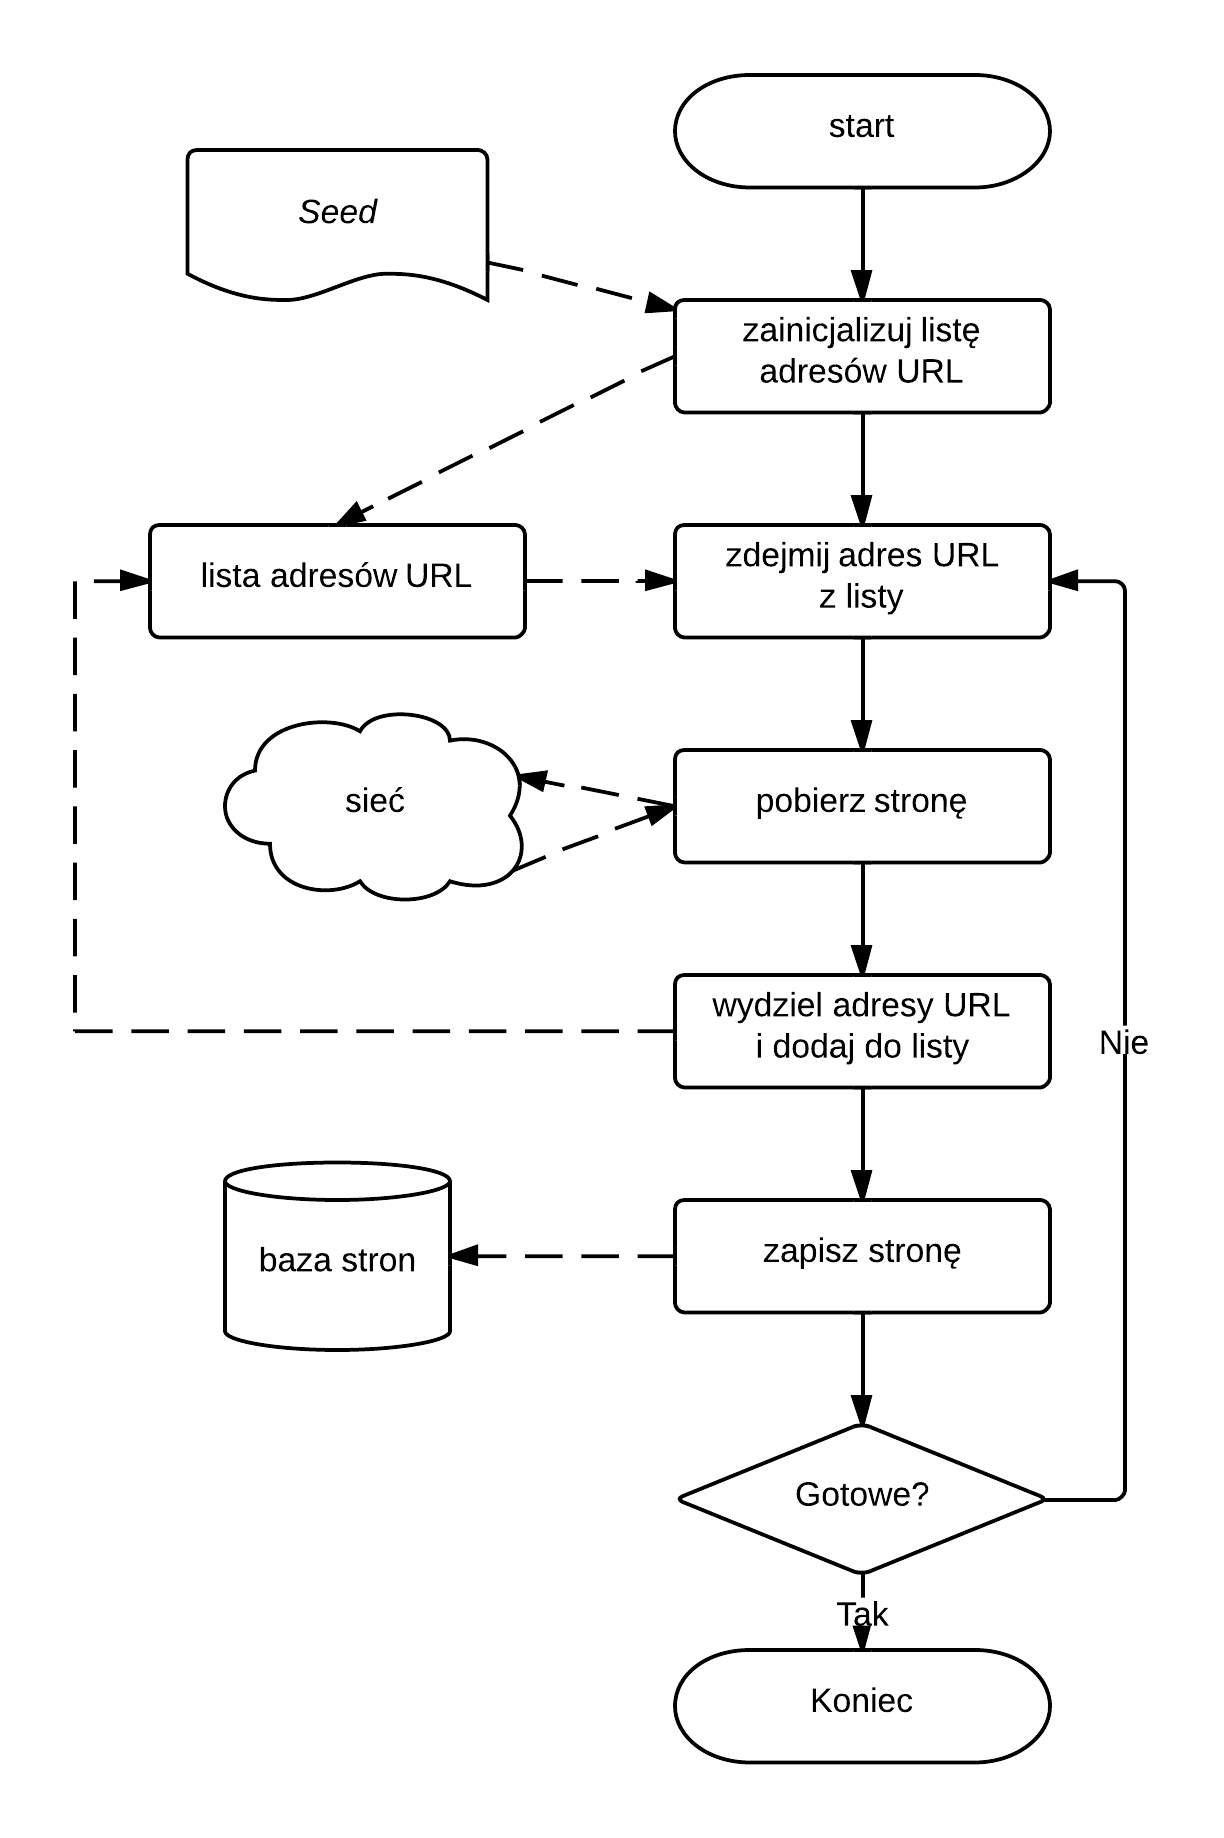
\includegraphics[scale=0.3]{spider_algorithm}
    \caption{Schemat blokowy algorytmu robota internetowego.}
\end{figure}

%%-----------------------------------------------------------------------------------------------------------------------------------------------------

\begin{figure}
    \centering
    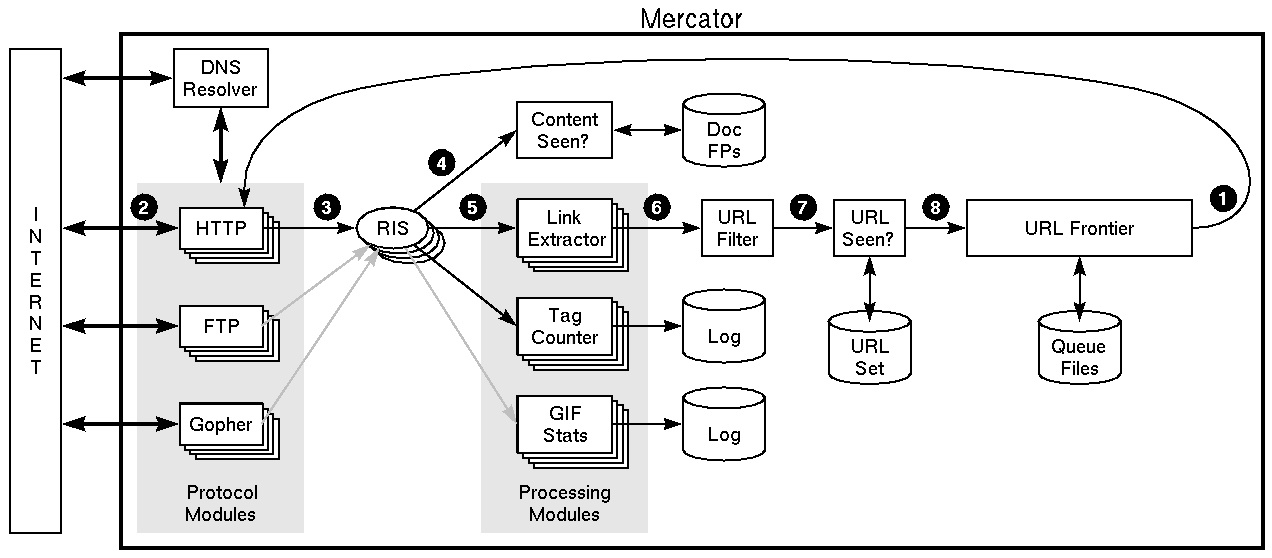
\includegraphics[scale=0.3]{mercator}
    \caption{Schemat crawlera Mercator, implementującego m.in. cache DNS.}
\end{figure}


%%-----------------------------------------------------------------------------------------------------------------------------------------------------

\subsection{Uwagi implementacyjne}
\label{subsec:uwagiImplement}

W związku z ilością scenariuszy możliwych do napotkania przy trawersowaniu sieci, jak i dużą ilością danych, która program przetwarza,
stosowane są dodatkowe zabiegi, zwiększające szanse poprawnego działania aplikacji.
\begin{enumerate}
    \item Stosowanie ścisłej kontroli nad ściąganiem stron: ograniczenie czasu trwania połączenia(stosowanie \emph{timeoutów}),
          określenie górnej granicy ilości danych pobieranych z jednej strony(np. do 50 KB), wykrywanie nieskończonych pętli przekierowań,
          logowanie błędów(przekroczenie czasu połączenia, błędne kody odpowiedzi itd.).
    \item Preprocessing pobranych źródeł, mający na celu eliminację częstych błędów występujących na stronach, takich jak np. niedomknięte tagi.
          Wykrycie kodowania i próba jego normalizacji - np. kodowanie wszystkich pobranych źródeł po stronie crawlera w formacie UTF-8.
          Na tym etapie można przeprowadzić również usuwanie słów nie niosących ze sobą istotnych treści(tzw. \emph{stopwords}), takich jak 
          np.~wyrazy ``a'', ``aby'', ``ach'', ``aczkolwiek'', ... itd. Stosowane są również inne formy przetwarzania danych, takie jak
          \emph{lematyzacja}~sprowadzenie do podstawowej formy  gramatycznej i 
          \emph{stemming}~utworzenie tzw. rdzenia słowa, części wspólnej słów niosących podobną informację \cite{lemStem}.
    \item Doprowadzenie linków do postaci kanonicznej. Przede wszystkim należy zapewnić przedstawienie wszystkich URLi w postaci aboslutnej. Ponadto stosowane
          są heurystyki związane np. z usuwaniem numeru portu, o ile figuruje w danym adresie, pozbywaniem się nieznaczących sufiksów oznaczających 
          typ dokumentu(np. .html), czy usuwanie tzw. fragmentu - części adresu następującej po znaku ``\#''.
    \item Unikanie tzw. pułapek na pająki (ang. \emph{spide-traps}). \emph{Pułapka na pająki} to strona, która generuje dynamicznie nieskończenie wiele 
          adresów URL prowadzących do niej samej \cite{spiderTraps}. Przykładem takiej witryny jest aplikacja kalendarza, który generuje linki do stron
          przedstawiających poprzednie lub następne przedziały czasu. Aby uniknąć nieskończonej pętli stosuje się różnego rodzaju heurystyki,
          np.~określa się górny limit ilości pobrań z danej domeny. Ma to jendak negatywny wpływ na aktualność informacji pobieranych ze stron
          o skończonej liczbe odnośników. Wpadnięcie wydajnego crawlera w taką pułapkę powoduje znaczne obciążenie serwerów i może być nawet interpretowane
          przez administratorów strony - pułapki jako atak denial of service \cite[s. 322]{webMining}.
    \item Wprowadzenie wielu wątków/procesów. Jak wspominano wcześniej, czas sekwencyjnego pobierania stron zależy w dużym stopniu od szybkości pobierania
          danych. Również, przy dużej ilości informacji, kosztowne może stać się również zapisaywanie danych na dysku. Jednym ze sposobów skrócenia
          czasu uzyskiwania nowych danych jest zastosowanie wielu równoległych wątków lub procesów, pobierających i przetwarzających dane niezależnie
          od siebie. Następuje wtedy jedynie konieczność synchronizacji dostępu i modyfikacji zarówno listy oczekujących do pobrania adresów URL. Takie
          podejście może w prosty sposób przyspieszyć działanie oprogramowania od 5 do 10 krotnie \cite[s. 323]{webMining}.
          
          Innym ulepszeniem, które może zostać wprowadzone do wielowątkowej architektury, jest pobieranie danych w sposób asynchroniczny. Pozwala to na 
          lepsze wykorzystanie dostępnej przepustowości sieci, niż w przypadku połączeń synchronicznych. Aby ograniczyć czas spędzony na translacji adresów
          URL na adresy IP wprowadza się specjalny serwis wykonujący ją zawczasu dla adresów URL oczekujących w kolejce i cache'ujący rezultaty.
          
\end{enumerate}

%------------------------------------------------------------------------------------------------------------------------------------------------------

\section{Ocena zbioru pobranych stron}
\label{sec:ocenaStron}

Oprócz efektywnego sposobu pobierania informacji z sieci, ważne jest również zrozumienie cech posiadanego zbioru stron internetowych i jego ewaluacja.
W tym przypadku dąży się zarówno do minimalizacji nieaktualnych informacji o witrynach internetowych, jak i do maksymalizacji ilości informacji o stronach
w ogóle. Szczególnie ważne jest szybkie reagowanie na zmiany(dodanawanie nowych dokumentów, edycję i usuwanie istniejących), które w wypadku sieci postępują
nadzwyczaj gwałtownie.

\subsection{Świeżość i wiek}
\label{subsec:swiezoscWiek}
Szczególnie ważnym zagadnieniem jest \textbf{świeżość} (ang. \emph{freshness}) \cite{webMining,webCrawling}. Miara ta jest określona dla pobranej strony \emph{p} w chwili \emph{t} jako
    \begin{equation}
        F_p(t) = 
        \begin{cases}
            1 &\text{  jeżeli } p\text{ jest takie samo, jak lokalna kopia}\\
            0 &\text{ w przeciwnym wypadku}
        \end{cases}
    \end{equation}

Dla tej samej pary można określić również \textbf{wiek} (ang. \emph{age}) \cite{webCrawling}, dany zależnością:
\begin{equation}
        A_p(t) = 
        \begin{cases}
            0 &\text{  jeżeli } p\text{ nie jest modyfikowane w chwili }t\\
            t - \text{czas modyfikacji } p &\text{ w przeciwnym wypadku}
        \end{cases}
    \end{equation}
    
W zależności od podjętych założeń stosuje się różne algorytmy selekcji dokumentów do ponownego odwiedzenia.

%------------------------------------------------------------------------------------------------------------------------------------------------------


\subsection{Algorytmy odświeżania zbioru dokumentów}
\label{sec:odswStron}

Pierwszy z przedstawionych algorytmów dąży do zminiejszenia liczby stron, które moga być nieaktualne. W tym modelu nie ma znaczenia historia historia
zmian zapisanej strony, wszystkie dokumenty odświeżane są z taką samą częstotliwością. Wiąże się to z utrzymywaniem dobrej średniej \textbf{świeżości},
\cite{freshAge} kosztem dopuszczenia możliwości posiadania nieaktualnych wersji pewnych nadzwyczaj często zmieniających się stron. 

Można również stosować inne podejście, które głosi, iż częstotliwość pobierania strony powinna być proporcjonalna do częstotliwości jej zmian w czasie.
Wprawdzie takie podejście sprawdza się dla witryn edytowanych regularnie, jednak nadużywane prowadzi do zbyt częstych, nieprzynoszących nowych informacji, 
odwiedzin adresów historycznie zmieniających się z dużą częstotliwością. \cite{freshAge}.

Mimo, iż pierwsze podejście jest bliższe optymalnemu, najlepsze rezultaty daje określenie rozkładu prawdopodobieństwa zmian dla poszczególnych witryn i 
dostosowywanie częstotliwości pobierania informacji z tych źródeł do otrzymanych rezultatów \cite{webCrawling}.

%------------------------------------------------------------------------------------------------------------------------------------------------------

\section{Charakterystyka zmian sieci w czase}
\label{sec:zmianySieci}

Poniżej przytoczona zostaje zbiorcza charakterystyka zmian w różnych podzbiorach sieci, uzyskana z \cite{webCrawling}.

\begin{table}[!h]
\caption{Zbiorcze dane dotyczące różnych badań zmian zachodzących w sieci.}
\begin{tabular}{llr}
\hline
\cline{1-2}
Podzbiór    & Obserwacje \\
\hline
360 losowych stron & mediana życia strony\(\approx\) 2.5 roku, \\
&33\% było wciąż dostępnych po 6 latach \\
\hline
500 stron & mediana życia strony \(\approx\) 4.5 roku \\
(arykułów naukowych on-line)&\\
\hline
2 500 stron & średnia długość życia \(\approx\) 50 dni \\
& mediana wieku \(\approx\) 50 dni \\
\hline
4 200 stron & mediana życia strony \(\approx\) 4 lat \\
(artykułów naukowych on-line) &\\
\hline
720 000 stron & średnia długość życia między 60, a 240 dni.\\
& 40\% stron w domenie \texttt{.com} zmienia się codziennie \\
& 50\% stron w domenach \texttt{.gov} i \texttt{.edu} pozostaje bez zmian\\
& przez 4 miesiące \\
\hline
950 000 stron & średni wiek między 4 dniami, a 4 miesiącami.\\
& Strony o dużej iości linków wskazujących na nie\\
& zmieniane częściej.\\
\hline
4 miliony stron & 8\% tygodniowy przyrost nowych stron\\
& 62\% stron tygodniowo dodaje nową treść\\
& 25\% tygodniowy przyrost nowych linków\\
& 80\% zmian jest niewielka\\
\hline
150 milionów stron & w 10 tygodniowym okresie 65\% stron\\
&pozostaje bez zmian\\
& na 30\% stron zachodzą jedynie niewielkie zmiany\\
& duża wariacja dostępności, w zależności od domeny\\
\hline
800 milionów stron & średnia długość życia \(\approx\) 140 dni\\
\hline
\end{tabular} 
\end{table}

Jak widać dynamika zmian w sieci zależy w dużym stopniu od indywidualnych witryn, ich miejsca w grafie oraz
celu, któremu służą. Praktycznie uniemożliwia to skonstruowanie ogólnego algorytmu odświeżającego posiadaną
kolekcję danych w sposób optymalny.

%------------------------------------------------------------------------------------------------------------------------------------------------------

\section{Kwestie etyczne}
\label{sec:etyczne}
Jak wspomniano wcześniej, crawlery używane są w wielu przydatnych zastosowaniach. W związku z tym inwestuje się wiele czasu i pracy w zoptymalizowanie
ich działania, od prostych zabiegów pobierania stron asynchronicznie, po zaawansowane technki modelowania rozkładu prawdopodobieństwa zmian na stronie.
Nie należy jednak zapominać, iż działalność prfesjonalnych, bardzo wydajnych robotów internetowych nie pozostaje obojętna dla innych użytkowników 
sieci. Ruch generowany w ten sposób może znacznie obciążać serwery pobieranych stron, powodując kłopoty dla ich administratorów i klientów.
Z tego powodu wprowadzono podstawowe zasady, którymi powinien kierować się każdy projektant oprogramowania trawersującego sieć. W momencie pisania
tej pracy nie mają one podstaw prawnych, ale łamiąc je notorycznie można liczyć się z potępieniem środowiska i poważniejszymi konsekwencjami, jak np.~zablokowaniem
puli adresów IP, z których korzysta nieposłuszny robot.

%------------------------------------------------------------------------------------------------------------------------------------------------------

\subsection{Identyfikacja}
\label{subsec:identyfikacja}

Administratorzy stron zazwyczaj zbierają informacje o ruchu, unikalnych użytkownikach, w których dane o działalności robotów nie są zazwyczaj przydatnymi
informacjami. Aby ułatwić identyfikację robotów, zaleca się umieszczenie w polu nagłówka zapytania HTTP \texttt{user-agent} nazwy crawlera i adresu
strony internetowej zawierającej infomracje o samym robocie oraz dane kontaktowe organizacji odpowiedzialnej za jego działanie.

%------------------------------------------------------------------------------------------------------------------------------------------------------

\subsection{Robot exclusion protocol}
\label{subsec:robotExcl}

W celu zapewnienia kontroli nad zasobami, do których dostęp mają roboty internetowe, wpropwadzono protokół podstron wykluczonych z indeksowania
\emph{ang. robot exclusion protocol}. Przyjmuje on formę statycznej strony internetowej serwowanej przez lokalny dla adres URL 
\url{/robots.txt} \cite{robotsTxt}. Każda linia powinna mieć następujący format: \texttt{<pole>:<opcjonalnaspacja><wartosc><opcjonalnaspacja>}.
Wg oficjalnej strony \cite{robotsTxt} \texttt{pole} może być zasąpione przez dwa ciągi znaków:
\begin{itemize}
    \item \texttt{User-agent:} - ciąg znaków odnoszący się do wartość nagłówka \texttt{user-agent} w zapytaniu. Podana dalej wartość identyfikuje
     poszczególne roboty, lub ich grupy. Oznaczanie grup robotów jest możliwe dzięki znakowi szczególnemu ``*'', który oznacza zero lub więcej
     wystąpień dowolnego znaku. Po linii zawierającej to pole następuje jedna lub więcej reguł dostępu do witryny. 
    \item \texttt{Disallow:} - dyrektywa odnosząca się do stron, których crawler nie powinien odwiedzać. Wartość specyfikuje pojedynczy adres URL, lub
     ich grupę wyłączoną z indeksacji.
\end{itemize}
Plik \url{robots.txt} może zawierać również komentarze, rozpoczynane są one znakiem ``\#''. Wszystkie znaki następujące później są ignorowane.
Dodatkowe reguły, respektowane przez niektóre roboty znaleźć można na ich stronach internetowych. Dla przykładu strona \url{https://developers.google.com/webmasters/control-crawl-index/docs/robots_txt}
przybliża sposób parsowania pliku \url{robots.txt} przez robota internetowego firmy Google. Ponadto wprowadza ona możliwość grupowania ciągów identyfikujących
pole \texttt{user-agent} i stosowanie zbioru reguł do całej grupy. Wprowadzona zostaje również dyrektywa \texttt{allow} pozwalająca wyszczególnić
strony, które robot może odwiedziać.

Poniżej znajdują się przykłady zastosowania przedstawionych wcześniej reguł, zaczerpnięte z \cite{robotsTxt}:

\begin{lstlisting}[frame=single]
# robots.txt for http://www.example.com/

User-agent: *
Disallow: /cyberworld/map/
Disallow: /tmp/ # these will soon disappear
Disallow: /bar.pdf
\end{lstlisting}

W tym przypadku żaden robot nie powinien odwiedzać adresu URL zaczynającego się od \url{/cyberworld/map/}, \url{/tmp/} lub \url{/bar.pdf}.

\begin{lstlisting}[frame=single]
User-agent: cybermapper
Disallow:

# go away
User-agent: *
Disallow: /
\end{lstlisting}

Natomiast ten plik pozwala na dostęp do strony tylko robotowi \texttt{cybermapper}.

Ograniczanie dostępu można uzyskać również poprzez umieszczenie w meta tagach HTML klucza \texttt{robots} i wartości
\texttt{noindex} zabraniającej indeksowania danego dokumentu i\textbackslash lub \texttt{nofollow} zabraniającej ściąganie stron linkowanych w 
dokumencie. Natomiast wartość \texttt{nocache} pozwala na pobranie i indeksację dokumentu, jednak nie wyraża zgody na pokazywanie lokalnej kopii
użytkownikom usługi wykorzystującej crawler.

%------------------------------------------------------------------------------------------------------------------------------------------------------

\subsection{Minimalny czas pomiędzy zapytaniami}
\label{subsec:minCzas}
Aby zniwelować obciążenie związane z działalnością crawlerów wprowadza się wymóg minimalnej ilości czasu, która musi upłynąc między dwoma
zapytaniami do tej samej domeny. Spotykane w literaturze propozycje wahają się od 60 do 1 sekundy. Niektóre roboty stosują algorytmy adaptacyjne,
uzależniające odstęp między kolejnymi zapytaniami od szybkości odpowiedzi serwisu \cite{webCrawling}.







